\begin{center}
    
    \resizebox{!}{.8cm}{
        \textbf{Óptica}        
    }
    \section{Noções de Óptica Ondulatória}
\end{center}
\begin{flushright}
    
     
    \rule{.33\textwidth}{.5pt}
    \renewcommand{\thefootnote}{\fnsymbol{footnote}}
    \par\noindent Por: Rodrigo Nascimento\footnote[2]{Estágio Curricular Obrigatório III -- ESC3003 (UDESC).} 
\end{flushright}


\section*{Introdução}       

O que é a Luz, como se propaga e qual a sua natureza, são os temas centrais da Óptica. Neste módulo de ensino, iremos estudar os aspectos mais elementares da propagação luminosa, que já eram parcialmente conhecidos desde a antiguidade.

A óptica se ramifica em diversas áreas de estudo, no ENEM tem-se basicamente apenas duas ramificações, sendo elas:
\begin{itemize}
    \item \textbf{Óptica Geométrica:} A luz é estudada como raios que percorrem trajetórias retilíneas. Fenômenos como a reflexão e a refração são observados, além disso, estuda-se também a formação de imagens em espelhos e lentes;
    \item \textbf{Óptica Física ou Ondulatória:} A luz é estudada como uma onda, os fenômenos como difração, interferência e polarização também aparecem naturalmente.
\end{itemize}

\setlength\intextsep{-20pt}
\begin{wrapfigure}[5]{l}{0.48\textwidth}
    \centering
    \begin{mybox}[colback=white, colframe=cyan,colbacktitle=cyan!85!cyan,]{Mais sobre!}
        Há diversos vídeos na plataforma YouTube que tratam sobre o tema, um deles pode ser encontrado \href{https://youtu.be/oSUHXeiaQ98}{aqui}.
    \end{mybox}    
\end{wrapfigure}

\noindent Os fenômenos da óptica geométrica, estão de acordo com a \emph{teoria corpuscular da luz}, creditada (erroneamente) à Isaac Newton (1643-1727). Uma segunda teoria, a \emph{teoria ondulatória}, foi proposta principalmente por Christian Huygens (1629-1695), Robert Hooke (1635-1703) e Thomas Young (1773-1829). Estes dois modelos formaram o palco para intensas discussões entre meados dos séculos XVII e XVIII.

A seguir falaremos um pouco sobre o conceito de ondas, para que possamos compreender corretamente os fenômenos luminosos.

\section*{Ondas}
\label{sec:nocoes-basicas-ondas}
Onda é o fenômeno causado pela perturbação de uma região do espaço ou um campo físico, propaga-se através desta uma região, a que chamamos de \emph{meio}, numa determinada velocidade. Um exemplo bastante comum, são as ondas do mar, causadas principalmente pelo deslocamento das massas de ar, propagam-se em direção à costa. Outros exemplos de ondas são: o som, a luz, os sinais de comunicação (rádio, televisão, celular e etc), os terromotos, dentre outros.

\begin{mybox}[colback=white, colframe=amarelo,colbacktitle=amarelo!85!amarelo,]{Conceituando}
    \emph{Uma onda pode ser compreendida como uma "perturbação" que se propaga de um ponto a outro, com velocidade definida.}
\end{mybox}

Neste sentido, fala-se de onda quando essa perturbação ocorre \emph{sem} que haja transporte de matéria, ou seja, em geral ondas só transportam energia!

\subsection*{Tipos de Ondas}
Pode-se classificar as ondas em quatro tipos:
\begin{enumerate}
    \item \textbf{Ondas Mecânicas:} Existem apenas num meio material dependendo dele para se propagar, como exemplo: ondas sonoras, ondas do mar e terremotos.  
    \item \textbf{Ondas Eletromagnéticas:} Não precisam de um meio material para existir ou se propogar, propagam-se tanto no vácuo como em meios materiais são exemplos de ondas eletromagnéticas: luz, microondas, rede wireless, sinal de GPS e etc.
    \item \textbf{Ondas de Matéria:} São mais comuns em laboratórios de pesquisa em Física Quântica e Teoria de Campos, estão associadas ao átomo e suas partículas elementares como: elétron, próton, bósons e etc.
    \item \textbf{Ondas Gravitacionais:} Ondulações geradas por colisões violentas entre corpos celestes, se propagam pelo espaço-tempo.
\end{enumerate}
As ondas ainda podem ser classificadas quanto a sua direção de propagação, sendo elas:
\begin{itemize}
    \item \emph{Unidimensionais:} Propagam-se em apenas uma direção, como por exemplo, as ondas em uma corda.
    \item \emph{Bidimensionais:} Com direção de propagação em um plano ou uma superfície, tal como as ondas num lago ou os terromotos.
    \item \emph{Tridimensionais:} Se propagam em todas as direções, como por exemplo o som e a luz. 
\end{itemize}
E por fim, também podem ser classificadas quanto a direção de vibração ou oscilação, sendo chamadas de:
\begin{itemize}
    \item \emph{Transversais:} Se originadas por oscilações perpendiculares à direção de propagação (ondas no mar, luz e ondas numa corda).
    \item \emph{Longitudinais:} Quando se propagam na mesma direção de oscilação (som).
\end{itemize}
Para o caso da luz, podemos dizer então que:
\begin{mybox}[colback=white, colframe=amarelo,colbacktitle=amarelo!85!amarelo,]{Conceituando}
    \emph{A Luz é uma onda eletromagnética, tridimensional transversal que propaga-se a uma velocidade constante sendo o valor da sua velocidade no vácuo $c=299\;792\;459\mps$ ou, aproximadamente $3,0\times 10^{8}\mps$.}
\end{mybox}

 \subsection*{Comprimento de onda}

Algumas grandezas são fundamentais para a descrição correta da onda, uma delas é o seu \emph{comprimento de onda} representado geralmente pela letra grega \emph{lambda} $\lambda$.

 \setlength\intextsep{-20pt}
 \begin{wrapfigure}[16]{l}{.6\textwidth}
    \centering
    \begin{mybox}[colback=white, colframe=deepred,colbacktitle=deepred!85!deepred,]{Comprimento de Onda ($\lambda$)}
        O \emph{comprimento de onda} $\lambda$ é a distância paralela à direção de propagação da onda, entre repetições da forma da onda.
        \tcblower
        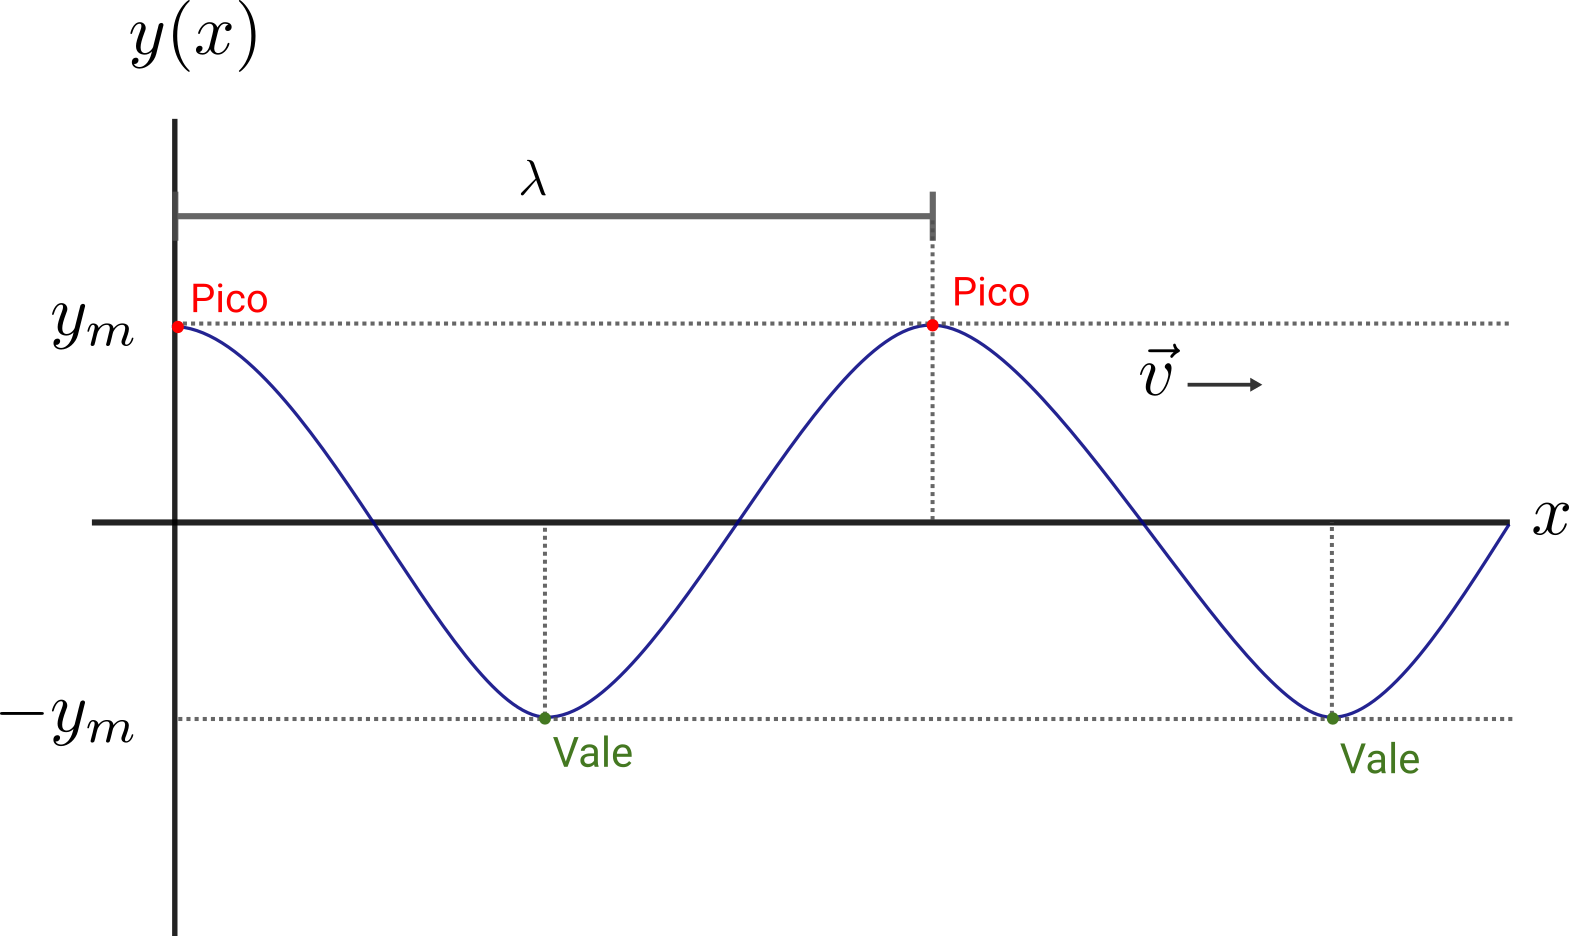
\includegraphics[width=1\textwidth]{img/lambda-1.png}
        \caption{Onda propagando-se em uma corda, paralela à direção do eixo $x$}
        \label{fig:comprimento-onda-corda} 
    \end{mybox}            
 \end{wrapfigure}

\noindent Imagine por exemplo, uma \emph{onda mecânica transversal unidimensional} propagando-se numa corda ao produzirmos alguns pulsos para cima e para baixo.

\noindent A \autoref{fig:comprimento-onda-corda} ilustra aproximadamente o que pode acontece com relação ao formato da onda em função do deslocamento em $x$ das frentes de onda (pulsos) produzidas.

\noindent Os pontos da corda que alcançam os pontos mais altos no eixo $y$ são os \emph{picos}, também chamados de \emph{Amplitude Máxima da Onda} ($y_m$), já os pontos mais baixos os \emph{vales}, são conhecidos como as \emph{Amplitudes Mínimas da Onda} ($-y_m$).

\noindent A distância entre dois picos locais ou (\emph{máximos consecutivos}), é igual a distância entre dois vales locais (\emph{mínimos consecutivos}), a essa medida chamamos de \textbf{comprimento de onda} $\lambda$. Tem unidade de distância (\emph{metro-$\m$, centímetro-$\cm$, nanômetro-$\nm$ e etc}).

       
\subsection*{Período}
\setlength\intextsep{-10pt}
\begin{wrapfigure}[21]{r}{.6\textwidth}
    \centering
    \begin{mybox}[colback=white, colframe=deepred,colbacktitle=deepred!85!deepred,]{Período de uma Onda ($T$)}
        O \emph{período} $T$ de oscilação de uma onda, é o tempo necessário para que a onda complete um ciclo, análogo ao período de oscilação de um pêndulo simples.
        \tcblower
        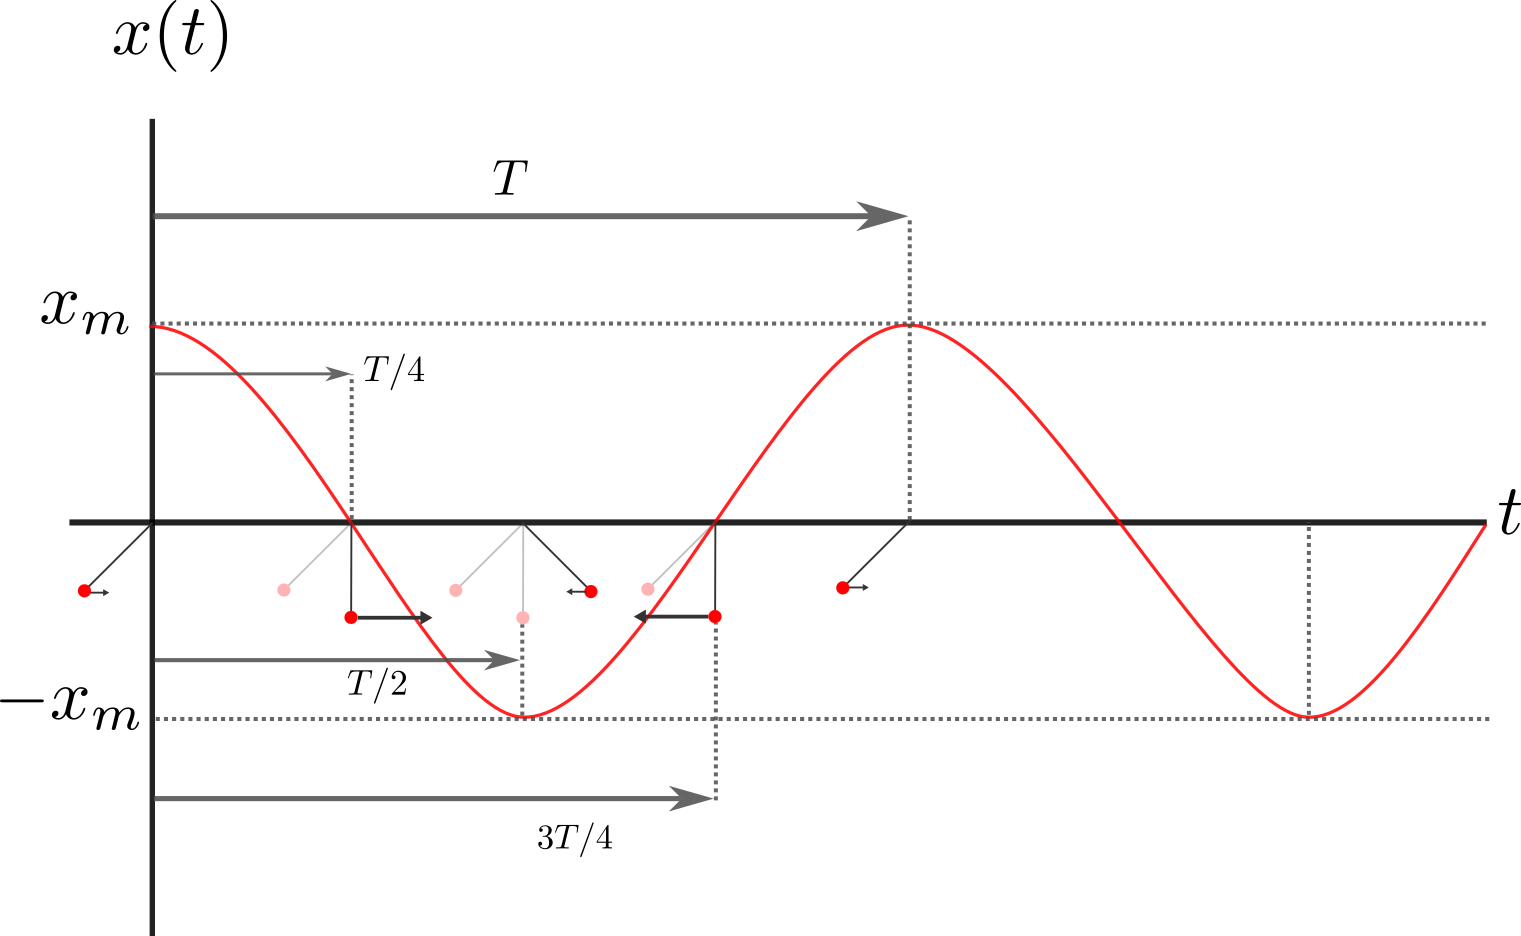
\includegraphics[width=1\textwidth]{img/periodo-1.png}
        \caption{No gráfico $x(t)$, tem-se o esquema de oscilação de um pêndulo que parte de uma posição $x_m$, vai até a posição oposta $-x_m$ e retorna a sua posição inicial.}
        \label{fig:periodo-onda-corda} 
    \end{mybox}            
\end{wrapfigure}       
Outra grandeza fundamental para a descrição de uma onda, é o seu \emph{período de oscilação}, utiliza-se geralmente a letra maiúscula $T$ para representá-lo. Na \autoref{fig:periodo-onda-corda} à direita, representamos o gráfico de um pêndulo oscilando no tempo, supondo que o pêndulo é colocado para oscilar a partir de uma posição qualquer $x_m$, após $T/4$ de tempo ele passa pela sua posição de equilíbrio em $x=0$, vai até a posição extremamente oposta $-x_m$ num tempo $T/2$, passa novamente pela sua posição de equilíbrio num tempo $3T/4$ e retorna ao ponto inicial em $x_m$. Ao tempo total em que o pêndulo fez este percurso, chamamos de \textbf{período de oscilação} $T$. Possui a unidade de tempo (\emph{segundo-$\s$}, \emph{milissegundo}-$\mathrm{ms}$ e etc).

As vezes estamos mais interessados em saber quantos ciclos uma onda conclui em um intervalo de tempo determinado. Por isso, defini-se uma grandeza física que tem uma relação imediata com o período da onda. Essa grandeza é a \emph{frequência da onda} caracterizada pela letra minúscula $f$.

\begin{mybox}[colback=white, colframe=deepred,colbacktitle=deepred!85!deepred,]{Frequência de uma Onda ($f$)}
    A quantidade de oscilações por unidade de tempo que um movimento oscilatório quelaquer conclui, dá-se o nome de frequência.
    \tcblower
    Matematicamente a frequência se relaciona com o período $T$ da seguinte forma:
    \begin{align}
        \label{eq:freq-periodo}
        f=\frac{1}{T}
    \end{align}
  \end{mybox}
A unidade de frequência é o inverso da unidade de tempo, o \emph{Hertz-$\Hz$} que equivale a $1\Hz=1\s^{-1}$.


\subsection*{Velocidade de uma Onda}
\label{sec:velocidade-da-onda}
Agora que já conhecemos algumas grandezas fundamentais de uma onda, podemos estabelecer uma equação para a sua \emph{velocidade de propagação} $v$. Da cinemática elementar, sabemos calcular a velocidade média de um objeto pela expressão:
\begin{align}
    v=\frac{\Delta S}{\Delta t}
\end{align}
Para uma onda que se propaga a uma distância igual ao seu comprimento de onda, $\Delta S=\lambda$ e num tempo igual ao seu período de oscilação $\Delta t=T$ de modo que a velocidade dessa onda é dada simplesmente por
\begin{align}
    \label{eq:velocidade-onda-T}
    v&=\frac{\lambda}{T}
\end{align}
ou ainda, como $f=1/T$, podemos fazer
\begin{align}
    v=&\lambda f
\end{align}


\section*{Propagação da Luz em um Meio}
\setlength\intextsep{-17pt}
\begin{wrapfigure}[21]{r}{0.55\textwidth}
\centering
\begin{mybox}[colback=white, colframe=deepred,colbacktitle=deepred!85!deepred,]{Lei da Reflexão}
    O raio refletido pertence ao mesmo plano do raio incidente e tem um ângulo de reflexão, igual ao ângulo do raio incidente.
    
    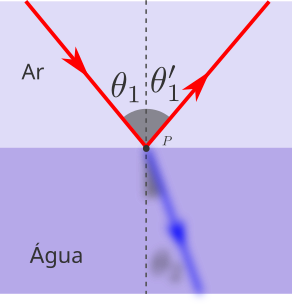
\includegraphics[width=1\textwidth]{img/reflexao.png}
    \caption{Lei da Reflexão}
    \label{fig:lei-da-reflexao}
    \tcblower
    \emph{Matematicamente:}
    \begin{align}
        \theta_1=\theta_1^{\prime }               
    \end{align}
  \end{mybox}    
\end{wrapfigure}
Vimos através da simulação do \emph{PheT}, que quando um feixe de luz incide sobre uma interface que separa dois meios físicos transparentes diferentes, a trajetória deste feixe sofre reflexão assim que encontra a interface, e um desvio ao entrar no meio. O ângulo que o raio incidente faz com a normal à superfície é sempre igual ao ângulo que o raio refletido também faz com a normal, está observação é conhecida normalmente como \emph{Lei da Reflexão}. A \autoref{fig:lei-da-reflexao} ao lado ilustra o caso.       

Já para o raio incidente e o refratado, podemos afirmar que, dependendo de em qual meio o feixe de luz está vindo e pra qual meio ele está indo, o feixe sofrerá um desvio que irá se aproximar da reta normal à superfície, ou se afastar dela, isto se deve ao fato de que a luz, ao passar de um meio para o outro, não altera a sua frequência, veremos mais adiante que como consequência disso, o comprimento de onda e a velocidade da onda sofrem mudanças na passagem entre os meios, provocando o desvio original de sua trajetória. A \autoref{fig:refracao} mostra o que observamos na simulação.

\vspace{5pt}
\begin{figure}[!ht]        
    \centering              
    \subfloat[Trajetória da luz partindo do ar para água \label{fig:refracao-a}]{
        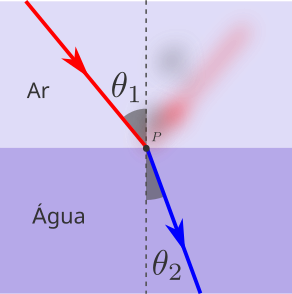
\includegraphics[width=.45\textwidth]{img/refracao-1a.png}
    }\hfill
    \subfloat[Trajetória da luz partindo da água para o ar \label{fig:refracao-b}]{
        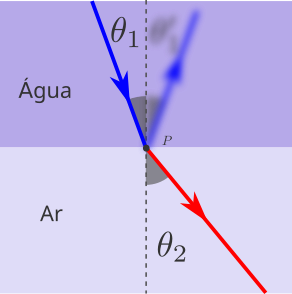
\includegraphics[width=.45\textwidth]{img/refracao-1b.png}
    }        
    \caption{Diagrama ilustrando um feixe de luz incidente e refratado na travessia entre dois meios ópticos ar e água, a seta indica a direção de propagação do feixe. Em (a) o feixe refratado está mais próximo da reta normal que o feixe incidente, o ângulo $\theta_1$ é maior que o ângulo $\theta_2$, já em (b) a situação se inverte quando invertemos os meios.}
    \label{fig:refracao}
  \end{figure}
\vspace*{20pt}

Embora seja possível explicar o fenômeno da refração pelo modelo corpuscular \emph{(possível porém nada simples)}, os resultados previstos diferem do que hoje é conhecido. A teoria corpuscular, prevê que a velocidade da luz deve ser \emph{maior} na água do que no ar, o que não é verdade! Por isso, o modelo ondulatório é mais correto para a descrição deste fenômeno, a seguir, usaremos o que aprendemos sobre ondas, para encontrar uma relação entre o ângulo incidente $\theta_1$ e o ângulo refratado $\theta_2$.


\subsection*{Índice de refração}        

Já vimos que os ângulos de incidência e refração, serão diferentes dependendo de cada meio físico e que tem relação direta com a velocidade da luz em cada meio. Convenientemente define-se uma grandeza auxiliar chamada de \textbf{índice de refração} $n$, cada meio possui um índice de refração associado e tem a ver com as propriedades físicas do material.

A relação entre o índice de refração e a velocidade da luz em um meio qualquer, é a razão entre a velocidade da luz em um meio conhecido e a velocidade da luz no meio em que a luz refrata. Um meio em que já se conhece bem como é a velocidade da luz é o vácuo e vale $c$ como já vimos anteriormente, por definição escreve-se o \textbf{índice de refração absoluto} como sendo:

\begin{align}
    n&=\frac{c}{v}
\end{align}
com
\begin{itemize}
    \item $n$: índice de refração absoluto;
    \item $c$: a velocidade da luz no vácuo ($c\simeq 3,0\times 10^8\mps$)
    \item $v$: a velocidade da luz no meio refratado.
\end{itemize}
\begin{mybox}[colback=white, colframe=darkpastelblue,colbacktitle=darkpastelblue!85!darkpastelblue,]{Exemplo Resolvido}
    \textbf{Calculando o índice de refração do ar:} Já foi determinado experimentalmente a velocidade da luz no ar, seu valor é $v_{\mathrm{ar}}=299\;705\;543,4\mps$. Calcular o índice de refração absoluto para o meio (ar), é só fazer a razão entre a velocidade da luz no vácuo $c=299\;792\;458\mps$ e $v_{\mathrm{ar}}$, segue que:

    \tcblower
    \begin{align}
        \begin{split}
            n_{\mathrm{ar}}&=\frac{c}{v_{\mathrm{ar}}}\\
            n_{\mathrm{ar}}&=\frac{299\;792\;458\mps}{299\;705\;543,4\mps}\\
            n_{\mathrm{ar}}&=1,00029\
        \end{split}
    \end{align}
    Por causa dessa proximidade entre a velocidade da luz no vácuo e no ar, convenciona-se que o índice de refração da luz no ar é $n_{\mathrm{ar}}=1,0$ igual ao do vácuo.        
\end{mybox}

\subsection*{Lei de Snell-Descartes}

Willebrord Snel van Royen (1580--1626) foi um matemático e astrônomo Holandês a quem atribui-se a descoberta da famosa \emph{Lei de Snell-Descartes} (também conhecida por \emph{Lei de Snell}).

Até a publicação do livro Optics de Huygens, a lei era atribuída somente a Descartes, porém, como a resolução de Descartes usou diversas suposições erradas, além de não haver nenhuma comprovação experimental, foram feitas acusações de que ele haveria forçado sua resolução a aproximar-se da de Snell. Contudo, nem Snell nem Descartes foram os primeiros a descobri-la e sim, um físico e matemático persa, que viveu entre os anos 940 e 1000 chamado Ibn Sahl, cujo o qual obteve resultados mais próximos dos que se conhece hoje em dia, porém sua pesquisa sobre a lei da refração não foi explicitada em seus trabalhos, ficando esquecida até meados do século XX.        

É possível deduzir a lei de Snell a partir dos conceitos estudados até aqui, para isso, vamos novamente relembrar da simulação feita na primeira aula.

Um feixe de luz propagando-se em um meio, que vamos chamar de meio \ding{192}, incide sobre uma superfície que separa este meio de um segundo, o meio \ding{193}. Sendo eles diferentes entre si, vimos que o feixe de luz tende a se comportar de duas formas: afastado-se da reta normal ao ponto em que houve o contato do feixe com a superfície, ou aproximando-se dela.

Vamos inicialmente supor que ao passar para o meio \ding{193}, o feixe aproxima-se da reta normal formando um ângulo de refração $\theta_2$. Se $\theta_1$ é o ângulo de incidência então $\theta_1>\theta_2$ por hipótese. A Figura\autoref{fig:snell-1} ilustra o caso.

\vspace{5pt}
\begin{figure}[!ht]        
    \centering              
    \subfloat[\label{fig:snell-1}]{
        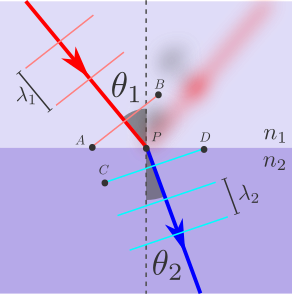
\includegraphics[width=.4\textwidth]{img/snell-1.png}
    }\hspace{20pt}
    \subfloat[\label{fig:snell-2}]{
        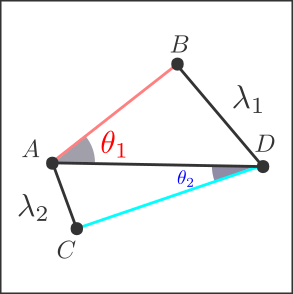
\includegraphics[width=.4\textwidth]{img/snell-2.png}
    }        
    \caption{Esquema representativo da refração da luz em dois meios diferentes. Em (a) o feixe propaga-se do meio \ding{192} para o meio \ding{193}, as frentes de onda estão representadas por retas perpendiculares à direção de propagação do feixe, como por exemplo a reta $\overline{AB}$ e $\overline{CD}$. Já em (b), tem-se um diagrama formado ligando os pontos $A$, $B$, $D$, $C$ e $A$ da Figura\autoref{fig:snell-1}, obtem-se assim, dois triângulos retângulos conectados pela hipotenusa $\overline{AD}$.}
    \label{fig:snell}
  \end{figure}        
  \vspace*{20pt}
  
  Na figura acima, o segmento de reta $\overline{AB}$ representa um pulso da onda luminosa no meio \ding{192}, a distância entre um pulso e outro nesse meio equivale a um comprimento de onda $\lambda_1$, o pulso seguinte encontra-se no meio \ding{193} e está representado pelo segmento de reta $\overline{CD}$, nesse meio a distância entre cada pulso é de $\lambda_2$. Cada parte do pulso $\overline{AB}$ ao entrar no meio \ding{193} é reorientado de forma que permaneça perpendicular à direção de propagação do feixe, assim, quando o ponto $A$ chegar no ponto $C$ o ponto $B$ também deve localizar-se no ponto $D$.

  Conectando os pontos $A$, $B$, $C$ e $D$, obtemos a Figura\autoref{fig:snell-2}. Do triângulo retângulo $\triangle ABD$ temos:
  \begin{align}
    \sin\theta_1&=\frac{\lambda_1}{\overline{AD}}
  \end{align}
  e do triângulo retângulo $\triangle ACD$ temos:
  \begin{align}
    \sin\theta_2&=\frac{\lambda_2}{\overline{AD}}
  \end{align}
  dividindo $\sin\theta_1$ por $\sin\theta_2$ chegamos a seguinte relação
  \begin{align}
    \begin{split}
        \frac{\sin\theta_1}{\sin\theta_2}&=\frac{\lambda_1}{\overline{AD}}\frac{\overline{AD}}{\lambda_2}\\
        \frac{\sin\theta_1}{\sin\theta_2}&=\frac{\lambda_1}{\lambda_2}
    \end{split}
  \end{align}
Algumas conclusões pode-se tirar da relação acima, por exemplo:
\begin{itemize}
    \item Se $\theta_1>\theta_2$ então $\lambda_1>\lambda_2$, ou seja, se o raio refratado sofre desvio aproximando-se da normal ($\theta_1>\theta_2$), o comprimento de onda da luz refratada é diminuído proporcionalmente ($\lambda_1>\lambda_2$).
    \item Analogamente, se $\theta_1<\theta_2$ então $\lambda_1<\lambda_2$, se o raio refratado sofre desvio afastando-se da normal ($\theta_1<\theta_2$), seu comprimento de onda sofre um alargamento ($\lambda_1<\lambda_2$). 
\end{itemize}


Isso explica alguns fenômenos que observamos cotidianamente por exemplo: porque o céu é azul durante o dia e vermelho ao entardecer, porque observamos as cores do arco-íris e a dispersão da luz em prismas, sempre numa certa ordem, veja a \autoref{fig:dispersao} a seguir:
\vspace{5pt}
\begin{figure}[!ht]        
    \centering              
    \subfloat[\label{fig:arco-iris}]{
        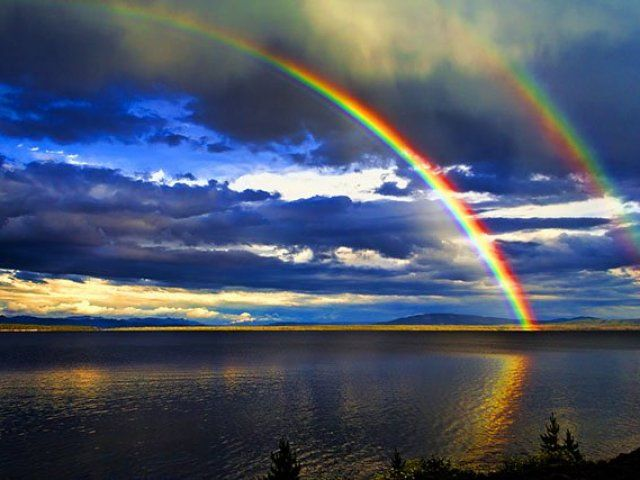
\includegraphics[width=.4\textwidth]{img/arco-iris.jpg}
    }\hspace{20pt}
    \subfloat[\label{fig:prisma-de-newton}]{
        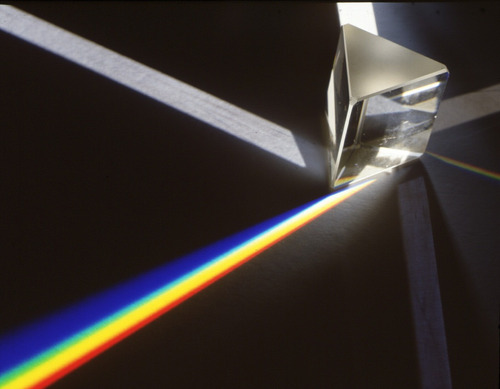
\includegraphics[width=.4\textwidth]{img/prisma.jpg}
    }        
    \caption{Fenêmeno de dispersão observado em (a) formação do arco-íris e (b) prisma de Newton. Se quiser saber sobre este assunto clique \href{https://www.bbc.com/portuguese/curiosidades-49906709}{aqui}}
    \label{fig:dispersao}
\end{figure}        
\vspace*{20pt}

Mas o que podemos dizer sobre a velocidade da luz? Sendo a luz um tipo de onda, vimos na seção \ref{sec:velocidade-da-onda} como calcular a sua velocidade em termos do comprimento de onda e da frequência da luz, $v=\lambda f$, se isso é verdade então podemos escrever a relação que encontramos como sendo a seguinte
\begin{align}
    \begin{split}
        \label{eq:lei-snell-frequencia}
        \frac{\sin\theta_1}{\sin\theta_2}&=\frac{\lambda_1}{\lambda_2}\\
        \frac{\sin\theta_1}{\sin\theta_2}&=\left(\frac{v_1}{f_1}\right)\left(\frac{f_2}{v_2}\right)
    \end{split}
\end{align}
Se tratando de luz monocromática, o feixe incidente é o mesmo feixe refratado no material, apenas com o comprimento de onda diferente, nesse caso a sua frequência de oscilação $f$ continua a mesma, ou seja $f_1=f_2=f$, \textbf{a frequência de uma onda monocromática nunca muda!} Então, reescrevemos a relação \eqref{eq:lei-snell-frequencia} como sendo:
\begin{align}
    \begin{split}
        \frac{\sin\theta_1}{\sin\theta_2}&=\left(\frac{v_1}{f}\right)\left(\frac{f}{v_2}\right)\\
        \frac{\sin\theta_1}{\sin\theta_2}&=\frac{v_1}{v_2}\label{eq:lei-snell-velocidades}
    \end{split}
\end{align}
E novamente,
\begin{itemize}
    \item Se o raio refratado se aproxima da normal $\theta_1>\theta_2$ a velocidade da onda refratada é \textbf{menor} que a velocidade da onda incidente $v_1>v_2$. Isto contraria a previsão feita pelo modelo corpuscular e por isso este modelo não é apropriado para descrever o fenômeno de refração!
    \item De outro modo, se o raio refratado se afasta da normal $\theta_1<\theta_2$, indicando que a velocidade do feixe de luz refratado é \textbf{maior} do que a velocidade do feixe incidente.
\end{itemize}
estes são os resultados previstos pela Lei de Snell-Descartes. Há uma forma de representar estes resultados em termos dos índices de refração de cada material, vamos retomar a equação \eqref{eq:lei-snell-velocidades} e reescrevê-la de uma forma em que tudo o que diz respeito a onda incidente fique de um lado da igualdade e tudo o que diz respeito a parte refratada da onda fique do outro lado
\begin{align}
    \begin{split}
        \frac{\sin\theta_1}{\sin\theta_2}&=\frac{v_1}{v_2}\\
        \frac{1}{v_1}\sin\theta_1&=\frac{1}{v_2}\sin\theta_2
    \end{split}
\end{align}
Agora é só multiplicarmos os dois lados da igualdade acima pela constate $c$ que representa a velocidade da luz, lembrando que a razão $c/v$ é definida como o índice de refração $n$, então
\begin{align}
    \begin{split}
        \frac{1}{v_1}\sin\theta_1&=\frac{1}{v_2}\sin\theta_2\\
        \frac{c}{v_1}\sin\theta_1&=\frac{c}{v_2}\sin\theta_2\\                                             
    \end{split}                                   
\end{align}
Assim, a forma mais conhecida da Lei de Snell-Descartes é dada por
\begin{align}
    \boxed{
        n_1\sin\theta_1=n_2\sin\theta_2
    } 
\end{align} 